\chapter{El procesador monociclo}

%%%%%%%%%%%%%%%%%%%%%%%%%%% Arquitectura de partida %%%%%%%%%%%%%%%%%%%%%%%%%%%%
\section{Descripción de la arquitectura de partida}

El código que describe la composición y funcionamiento internos del pipeline original se encuentra distribuido en cinco módulos, cada uno de los cuales modela una de las cinco etapas en las que se ha decidido segmentarlo. Además, existe un módulo superior dentro del cual se establece el conexionado entre las diferentes etapas y, por encima de este, un módulo en un nivel adicional en el que se definen las conexiones entre el agregado de las unidades funcionales del pipeline y la memoria, unificada, la cual alberga datos e instrucciones.

Se proporciona a continuación, en la Figura 4.1, un diagrama con el que se espera poder ayudar a comprender las relaciones entre los distintos componentes que conforman el computador.

\vspace{+0.3cm}
\begin{figure}[h]
  \centering
  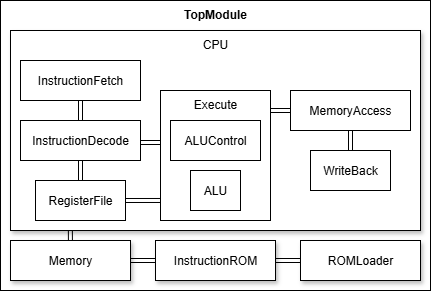
\includegraphics[width=0.7 \linewidth]{res/img/diagramas/5-arquitectura-global-blackbox/diagrama-arquitectura-blackbox.png}
  \caption{Diagrama de bloques de la arquitectura global del computador}
\end{figure}

\vspace{+0.1cm}
A continuación se indicarán los módulos que conforman el diseño de partida junto con una descripción tanto de la funcionalidad que modelan, como de las señales de entrada y salida que reciben y generan respectivamente. Además, cabe indicar que los ficheros de código fuente donde se encuentra definido cada módulo siguen la siguiente nomenclatura: \textit{«NombreModulo».scala}.

%%%%%%%%%%%%%%%%%%%%%%%%%%%%%%%%%%% TopModule %%%%%%%%%%%%%%%%%%%%%%%%%%%%%%%%%%
\subsection{TopModule}

\textit{TopModule} es el módulo en el que se describe el conexionado de los grandes bloques que conforman el computador, es decir, el núcleo, la memoria, el cargador y la ROM de instrucciones, cuyo funcionamiento interno e interoperabilidad serán descritos en los subapartados siguientes a este.

El módulo cuenta con una interfaz de entrada-salida cuyos puertos permiten observar el estado del banco de registros y de la memoria en cualquier momento, lo cual resulta de gran utilidad cuando se necesita depurar la ejecución de programas complejos que puedan sacar a la luz defectos en el diseño del pipeline, los cuales no hubieran podido ser detectados por medio de los tests convencionales que prueban el comportamiento individual de cada uno de los componentes que conforman el diseño global.

%%%%%%%%%%%%%%%%%%%%%%%%%%%%%%%%%%%% Memory %%%%%%%%%%%%%%%%%%%%%%%%%%%%%%%%%%%%
\subsection{Memory}

Tal y como se indicaba al comienzo de este capítulo sobre la arquitectura interna del computador, la memoria se encuentra unificada, albergando tanto instrucciones como datos, lo cual contribuye a simplificar el diseño global, haciendo posible que todas las operaciones sobre la memoria sean realizadas por medio de una misma interfaz, definida dentro de un único módulo (\textit{Memory}) que cuenta, además, con una instancia definida dentro del módulo \textit{TopModule}.

Sobre el código del módulo \textit{Memory}, en él se define la clase \textit{Memory} con la que se construyen tanto la memoria unificada del computador, como la interfaz a la que se conecta el módulo \textit{CPU} para habilitar la comunicación entre la memoria y los módulos que compomen el núcleo, más concretamente, \textit{InstructionFetch} y \textit{MemoryAccess}, que emplean los puertos definidos en la interfaz de la memoria para leer de manera independiente, y en paralelo, los datos e instrucciones que en ella se encuentran alojados.

A continuación se detallará el propósito de los puertos de entrada-salida del módulo. No obstante, dentro de la entrada-salida se define también un \textit{bundle} como una instancia de la clase \textit{RAMBundle}, definida dentro del mismo fichero donde se especifica la clase \textit{Memory}. Al instanciar esta clase se crea un \textit{Bundle} de Chisel, es decir, una agrupación de señales de entrada-salida, en este caso, relacionadas con la interacción con la memoria.

\subsubsection{Señales de entrada}

\begin{itemize}
  \item \textbf{\textit{instruction\_address}}: es un bus de 32 bits por donde la memoria recibe la dirección de la siguiente instrucción generada en el \textit{fetch}.
  \vspace{-0.2cm}
  \item \textbf{\textit{debug\_read\_address}}: se trata de otro bus de 32 bits por el que la memoria puede recibir direcciones arbitrarias en cualquier instante de tiempo con fines de depuración.
  \vspace{-0.2cm}
  \item \textbf{\textit{address@bundle}}: la utilidad de este puerto, definido dentro del \textit{bundle}, es indicar una dirección de memoria, cualquiera, para leerla o escribir en ella
  \vspace{-0.2cm}
  \item \textbf{\textit{write\_data@bundle}}: es un bus de 32 bits mediante el cual se indica un dato a escribir en memoria
  \vspace{-0.2cm}
  \item \textbf{\textit{write\_enable@bundle}}: una señal con la que habilitar o deshabilitar la escritura en memoria
  \vspace{-0.2cm}
  \item \textbf{\textit{write\_strobe@bundle}}: tal y como puede verse en la Figura 4.2, donde se muestra el código con el que se implementa la clase RAMBundle, el tipo de dato del puerto de entrada \textit{write\_strobe} es un vector. Cada elemento de este vector es un booleano que indica si la sección n-ésima de la palabra a escribir en memoria, donde $0 \le n < Parameters.DataWidth$, con $Parameters.DataWidth = 4$, deberá o no serlo. Por ejemplo, en las instrucciones de escritura de bytes individuales, el vector con el que se define el `strobe' deberá tener la siguiente forma para indicar que deberá escribirse el último de los 4 bytes que conforman el dato: \{0001\}.
\end{itemize}

\subsubsection{Señales de salida}
\begin{itemize}
  \item \textbf{\textit{instruction}}: la instrucción leída en la dirección \textit{instruction\_address}.
  \vspace{-0.2cm}
  \item \textbf{\textit{debug\_read\_data}}: el dato leído en la dirección \textit{debug\_read\_address}.
  \vspace{-0.2cm}
  \item \textbf{\textit{read\_data@bundle}}: el dato leído en la dirección \textit{address@bundle} con la máscara indicada en el \textit{strobe}.
\end{itemize}

\begin{figure}[h]
  \centering
  \begin{minipage}{0.9\linewidth}
    \begin{lstlisting}[style=scalaStyle]{}
class RAMBundle extends Bundle {
  val address       = Input(UInt(Parameters.AddrWidth))
  val write_data    = Input(UInt(Parameters.DataWidth))
  val write_enable  = Input(Bool())
  val write_strobe  = Input(Vec(Parameters.WordSize, Bool()))
  val read_data     = Output(UInt(Parameters.DataWidth))
}
    \end{lstlisting}
    \caption{Implementación de la clase RAMBundle}
  \end{minipage}
\end{figure}

%%%%%%%%%%%%%%%%%%%%%%%%%% InstructionROM y ROMLoader %%%%%%%%%%%%%%%%%%%%%%%%%%
\subsection{InstructionROM y ROMLoader}

Puede verse en el diagrama de la Figura 4.1 que el computador lo componen, además del núcleo y la memoria, dos piezas adicionales: \textit{InstructionROM} y \textit{ROMLoader}. Estos son dos módulos involucrados en la carga de binarios en memoria. El primero define internamente una rutina con la que se traslada el contenido del fichero binario resultante de un proceso de compilación cruzada, a un fichero de texto codificado en ASCII con el que puede inicializarse una memoria de Chisel, definida también a nivel interno dentro del módulo. Posteriormente, la lógica que define el comportamiento del módulo \textit{ROMLoader} se encarga de trasladar, palabra a palabra, los contenidos de la ROM de instrucciones a la memoria de la CPU, a partir de un punto de entrada recibido como parámetro.

Por último, el módulo \textit{ROMLloader} cuenta con una señal de salida con la que indica al módulo superior \textit{TopModule} que la carga del programa en memoria ha finalizado, con lo que la ejecución podría dar comienzo. Mientras la carga del programa sigue en curso, el \textit{bundle} de la memoria (\textit{Memory}) permanece conectado a un bundle definido dentro de \textit{ROMLoader}, de modo que pueda hacerse el volcado del contenido de la memoria definida dentro de \textit{InstructionROM}, a la memoria que empleará más adelante el core. Cuando el cargador finaliza su trabajo, se desacopla de la memoria y esta se conecta al core ya con el programa cargado y listo para ejecutar.

En la Figura 4.3 se proporciona el fragmento del código de la clase \textit{TOPModule} con el que se construye la lógica que define el comportamiento descrito en este último párrafo. Puede verse que el acoplamiento entre los \textit{bundles} del cargador y la memoria, o entre esta y el núcleo, se realiza por medio del operador ´$<>$´, con el que se realiza el conexionado de señales con el mismo nombre.

\vspace{+0.3cm}
\begin{figure}[h]
  \centering
  \begin{minipage}{0.9\linewidth}
    \begin{lstlisting}[style=scalaStyle]{}
when(!rom_loader.io.load_finished) {
  rom_loader.io.bundle <> mem.io.bundle
  cpu.io.memory_bundle.read_data := 0.U
}.otherwise {
  rom_loader.io.bundle.read_data := 0.U
  cpu.io.memory_bundle <> mem.io.bundle
}
    \end{lstlisting}
    \caption{Implementación de la clase RAMBundle}
  \end{minipage}
\end{figure}

%%%%%%%%%%%%%%%%%%%%%%%%%%%%%%%%%%%%% CPU %%%%%%%%%%%%%%%%%%%%%%%%%%%%%%%%%%%%%%
\subsection{CPU}

Este módulo constituye uno de los grandes bloques que conforma el computador, el núcleo, y en su interior se describe el conexionado entre los distintos bloques que modelan cada una de las etapas por las que pasa una instrucción cuando es leída de la memoria. El funcionamiento de estas etapas se describirá en los subapartados siguientes a este.

Además de este conexionado, se define una interfaz de entrada-salida con los siguientes puertos:

\subsubsection{Puertos de entrada}
\begin{itemize}
  \item \textbf{\textit{instruction}}: la instrucción leída de la memoria, en la dirección que genera el módulo \textit{InstructionFetch}.
  \vspace{-0.2cm}
  \item \textbf{\textit{instruction\_valid}}: una señal que controla el flujo de ejecución de nuevas instrucciones, en tanto que puede detener su lectura, paralizando el pipeline. Esta entrada se conecta al puerto de salida \textit{load\_finished} del cargador, con el que se indica que la carga de instrucciones en la memoria principal del computador ha finalizado, puediendo dar comienzo a la ejecución del programa.
  \vspace{-0.2cm}
  \item \textbf{\textit{debug\_read\_address}}: un bus de 5 bits por el cual puede indicarse el índice de un registro cuyo valor quiera conocerse. Esta dirección es recibida por medio de su correspondiente puerto de depuración en el módulo superior (\textit{TopModule}).
\end{itemize}

\subsubsection{Puertos de salida}
\begin{itemize}
  \item \textbf{\textit{debug\_read\_data}}: el puerto de depuración donde el núcleo deposita el contenido del registro solicitado.
  \vspace{-0.2cm}
  \item \textbf{\textit{instruction\_address}}: la dirección de la siguiente instrucción generada en el \textit{fetch}.
  \vspace{-0.2cm}
  \item \textbf{\textit{device\_select}}: el computador puede tener conectados hasta 8 dispositivos mapeados en memoria, cada uno de los cuales se identifica por medio de una etiqueta de 3 bits ($\log_2 8 = 3 bits$), y es este el puerto por medio del cual se indica el dispositivo con cuyo espacio de memoria se quiere interactuar. En la práctica este puerto carece de utilidad, puesto que el único dispositivo con cuya memoria puede trabajarse desde el núcleo es la propia memoria principal. No obstante, queda claro que este mecanismo resultaría muy conveniente si se quisiera dotar al computador de comunicación de entrada-salida con una mayor variedad de dispositivos.
\end{itemize}

%%%%%%%%%%%%%%%%%%%%%%%%%%%%%%% InstructionFetch %%%%%%%%%%%%%%%%%%%%%%%%%%%%%%%
\subsection{InstructionFetch}

En este módulo se describe el comportamiento de la fase de \textit{fetch}, donde se avanza el contador de programa a la siguiente instrucción sumándole 4 unidades\footnote{Recordemos que se trata de un sistema 32 bits direccionable a byte, por lo que la siguiente instrucción se encontrará alejada 32 bits (4 bytes) respecto de la actual}, siempre y cuando se de alguna de las dos circunstancias siguientes:

\begin{itemize}
  \item Que el cargador haya terminado de volcar el contenido de la ROM de instrucciones en la memoria principal de la CPU.
  \vspace{-0.2cm}
  \item Que el decodificador no haya determinado en el ciclo anterior que la instrucción en ese ciclo era un salto que debía tomarse.
\end{itemize}

En el primer caso el contador de programa permanecerá inmutable hasta el momento en que el cargador comunique la finalización del proceso de volcado y, en el segundo caso, el contador de programa tomará el valor del destino del salto.

\subsubsection{Señales de entrada}

\begin{itemize}
  \item \textbf{\textit{jump\_flag\_id}}: es un bit que indica si el valor del contador de programa deberá ser igual al valor actual más cuatro unidades o, por el contrario, la dirección de destino de un salto que debe ser tomado.
  \vspace{-0.2cm}
  \item \textbf{\textit{jump\_address\_id}}: una señal de 32 bits por donde se recibe la dirección de destino calculada en la ejecución de las instrucciones de salto.
  \vspace{-0.2cm}
  \item \textbf{\textit{instruction\_read\_data}}: la instrucción leída de la memoria en la posición del contador de memoria.
  \vspace{-0.2cm}
  \item \textbf{\textit{instruction\_valid}}: la señal con la que el cargador indica que su trabajo ha finalizado.
\end{itemize}

\subsubsection{Señales de salida}

\begin{itemize}
  \item \textbf{\textit{instruction\_address}}: la dirección de la instrucción a leer de la memoria en el siguiente ciclo.
  \vspace{-0.2cm}
  \item \textbf{\textit{instruction}}: la instrucción leída de la memoria en el ciclo actual. Se hace un \textit{passthrough}, es decir, una asignación directa, entre este puerto y el puerto \textit{instruction\_read\_data}.
\end{itemize}

Originalmente el código de este módulo se encontraba incompleto, puesto que carecía de la implementación de la lógica que establece el siguiente valor del contador de programa, es decir, el destino de un salto o la dirección de la siguiente instrucción en el programa. Esta lógica, mostrada en el código de la Figura 4.4, consiste en un multiplexor cuyo selector se conecta a la señal \textit{jump\_flag\_id}, y cuyas dos entradas son, por un lado, el destino de un salto recibido por el puerto \textit{jump\_address\_id} y, por otro lado, el valor del contador de programa más cuatro unidades (recordemos que se trata de una arquitectura de 32 bits).

\vspace{+0.3cm}
\begin{figure}[h]
  \centering
  \begin{minipage}{0.9\linewidth}
    \begin{lstlisting}[style=scalaStyle]{}
pc := Mux(io.jump_flag_id, io.jump_address_id, pc + 4.U)
    \end{lstlisting}
    \caption{Conexionado del contador de programa a la salida del multiplexor que determina su valor a cada ciclo en función de los saltos que se producen en el flujo de ejecución de los programas cargados en el computador}
  \end{minipage}
\end{figure}

%%%%%%%%%%%%%%%%%%%%%%%%%%%%%%% InstructionDecode %%%%%%%%%%%%%%%%%%%%%%%%%%%%%%
\subsection{InstructionDecode}

Como su nombre indica, esta es la clase que modela la lógica encargada de realizar la decodificación de las instrucciones recibidas desde el módulo de \textit{fetch} para elaborar el conjunto de señales que componen la palabra de control, por medio de las cuales se gobernará el comportamiento del resto de unidades funcionales en el pipeline, de modo que estas actúen conforme al significado de las instrucciones decodificadas.

Se trata quizás del módulo con mayor complejidad de entre todos de los que se compone el pipeline, y esto se debe al elevado número de casuísticas que deben contemplarse en la generación de la palabra de control, que son el resultado directo de la variabilidad en cuanto a formatos de instrucciones dentro del ISA, así como de la variabilidad en el conjunto de valores posibles que pueden tomar los campos definidos en estos formatos.

\subsubsection{Señales de entrada}

\begin{itemize}
  \item \textbf{\textit{instruction}}: la instrucción leída en la fase de \textit{fetch}.
\end{itemize}

\subsubsection{Señales de salida}

\begin{itemize}
  \item \textbf{\textit{regs\_reg\{1,2\}\_read\_address}}: las direcciones de los registros cuyos valores se emplearán en el cómputo de los resultados de instrucciones aritmético-lógicas, o en la determinación del cumplimiento de la condición de salto en las instrucciones de salto condicional.
  \vspace{-0.2cm}
  \item \textbf{\textit{ex\_immediate}}: ...
\end{itemize}

...TO-DO...